\documentclass[a4paper, 12pt]{article}

\usepackage{hyperref}
\usepackage[warn]{mathtext}
\usepackage[utf8]{inputenc}
\usepackage[T2A]{fontenc}
\usepackage[english,russian]{babel}
\usepackage{multirow}
\usepackage{float}
\restylefloat{table}
\usepackage{amsmath,amsfonts,amssymb,amsthm,mathtools}
\usepackage{indentfirst}
\DeclareSymbolFont{T2Aletters}{T2A}{cmr}{m}{it}
\usepackage{ gensymb }
\mathtoolsset{showonlyrefs=true}
\usepackage{euscript}
\usepackage{mathrsfs}
\usepackage[left=2cm,right=2cm,top=2cm,bottom=2cm]{geometry}
\usepackage{graphicx}
\usepackage{wrapfig}
\usepackage[rgb]{xcolor}
\hypersetup{
colorlinks=true,
urlcolor=blue
}
\usepackage{tikz}

\title{Лабораторная работа}
\author{Гисич Арсений Б03-102}
\date{2023}

\begin{document}

	\begin{center}
		{\large МОСКОВСКИЙ ФИЗИКО-ТЕХНИЧЕСКИЙ ИНСТИТУТ (НАЦИОНАЛЬНЫЙ ИССЛЕДОВАТЕЛЬСКИЙ УНИВЕРСИТЕТ)}
	\end{center}
	\vspace{5 cm}
	{\Large
		\begin{center}
			{\bf Лабораторная работа 4.1.2}\\[0.2 cm]
			Моделирование оптических приборов и определение их увеличения
		\end{center}
	}
	\vspace{4 cm}
	\begin{flushright}
		{\Large Выполнили: \\
			\vspace{0.2 cm}
			Гисич Арсений \\
			Данилов Иван \\
			\vspace{0.2 cm}
			Б03-102 \\}
	\end{flushright}
	\vspace{7 cm}
	\begin{center}
		Долгопрудный\\[0.1 cm]
		2023
	\end{center}
\thispagestyle{empty}

\section{Аннотация}

В данной работе были изучены модели зрительных труб (астрономической трубы Кеплера и земной трубы Галилея) и микроскопа, различными способами были определены их увеличения.

\section{Методика измерений}

\textbf{Центрирование линз.} При юстировке любых оптических приборов важно правильно центрировать входящие в систему линзы. Проходя через плохо
	отцентрированную систему линз, лучи света отклоняются в сторону и могут
	вообще не доходить до глаза наблюдателя. Центрировать линзы следует как
	по высоте, так и в поперечном направлении (для чего линзы крепятся на, поперечных салазках). Подробно с правилами центрировки Вы познакомитесь
	при выполнении задания.
	
\textbf{Юстировка коллиматора.} При составлении моделей телескопических
	систем необходимо иметь удалённый объект. В качестве такого объекта обычно используется бесконечно удалённое изображение предмета (шкалы осветителя), установленного в фокальной плоскости положительной линзы. Лучи,
	выходящие из одной точки предмета, пройдя через линзу, образуют параллельный пучок. Устройство такого рода называется \textit{коллиматором}.

Для юстировки коллиматора удобно использовать вспомогательную зрительную трубу, предварительно настроенную на бесконечность. Передвигая
	линзу коллиматора вдоль скамьи, добиваются появления резкого изображения предмета в окуляре зрительной трубы.
	
\textbf{Измерение фокусных расстояний линз.} Для того, чтобы сознательно
	моделировать оптические инструменты, нужно знать фокусные расстояния
	линз, которые могут быть использованы в качестве объектива или окуляра модели. Фокусные расстояния тонких положительных линз проще всего
	найти с помощью вспомогательной зрительной трубы, установленной на бесконечность. Работа выполняется так же, как при юстировке коллиматора.
	
При определении фокусного расстояния отрицательной линзы предметом
	служит изображение шкалы, которое даёт вспомогательная положительная
	линза.
  	
\section{Используемое оборудование}

\begin{enumerate}
    \item оптическая скамья;
    \item набор линз;
    \item экран;
    \item осветитель со шкалой;
    \item зрительная труба;
    \item диафрагма;
    \item линейка.
\end{enumerate}

\section{Результаты измерений и обработка данных}

%Параметры установки:
%\begin{description}
%\item{} $R_0 = 0,2~Ом$
%\item{} $R_и = 20~кОм$
%\item{} $C_и = 20~мкФ$
%\end{description}

\subsection{Центрировка элементов оптической системы}

Из набора линз требуется выбрать собирающие и рассеивающие линзы. Для этого нужно получить с помощью собирающих линз чёткое изображение удалённого объекта. Так как изображение получится в фокальной плоскости, можно оценить фокусное расстояние линзы. Результаты оценки фокусного расстояния линз представлены в таб.~\ref{tab1}. Если не удаётся получить чёткое изображение, значит линза рассеивающая.

\begin{table}[h!]
\begin{center}
\begin{tabular}{|c|c|}
\hline 
Номер линзы & Фокусное расстояние, см \\ 
\hline 
1 & 6 \\ 
\hline 
2 & 10 \\ 
\hline 
3 & 20,5 \\ 
\hline 
4 & 30 \\ 
\hline
5 & рассеивающая \\
\hline
\end{tabular} 
\end{center}
\caption{Оценка фокусных расстояний линз}
\label{tab1}
\end{table}

Для центрировки оптической системы сначала на оптическую скамью ставится одна собирающая линза. С помощью регулировки винтов рейтера выставляется чёткое изображение осветителя по центру экрана. Затем ставится следующая линза и процедура повторяется.

\subsection{Определение фокусных расстояний тонких линз с помощью зрительной трубы}

Поставим собирающую линзу на расстоянии от предмета, примерно равным фокусному. На небольшом расстоянии от линзы закрепим трубу, настроенную на бесконечность. Передвигая линзу вдоль скамьи, получим  в окуляре зрительной трубы изображение предмета --- миллиметровой сетки. Также проведём такие же измерения повернув линзу другой стороной к источнику. Результаты измерений представлены в таб.~\ref{tab2}.

\begin{figure}[h!]
\begin{center}
	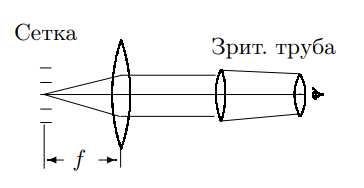
\includegraphics[width=0.6\textwidth]{plus_lens.png}
\end{center}
\caption{Определение фокусного расстояния собирающей линзы}
\label{fig:plus_lens}
\end{figure}

Для определения фокусного расстояния рассеивающей линзы сначала получим на экране увеличенное изображение сетки при помощи одной короткофокусной линзы. Измерим расстояние между экраном и линзой $a_0$. Разместим сразу за экраном трубу, настроенную на бесконечность. На место экрана поставим исследуемую рассеивающую линзу. Перемещая рассеивающую линзу, найдём в окуляре зрительной трубы резкое изображение сетки. Измерив расстояние между линзами $l$ найдём фокусное расстояние рассеивающей линзы $f = l - a_0$. Повернём рассеивающую линзу другой стороной к источнику и повторим измерения. Результаты измерений представлены в таб.~\ref{tab2}.

\begin{table}[h!]
\begin{center}
\begin{tabular}{|c|c|c|}
\hline 
Номер линзы & $f_{пр}$, см & $f_{обр}$, см \\ 
\hline 
1 & $7,5\pm0,1$ & $7,5\pm0,1$ \\ 
\hline 
2 & $11\pm0,1$ & $10,5\pm0,1$ \\ 
\hline 
3 & $18,7\pm0,1$ & $19,2\pm0,1$ \\ 
\hline 
4 & $28,5\pm0,1$ & $28,2\pm0,1$ \\ 
\hline
5 & $-13,0\pm0,1$ & $-11,0\pm0,1$ \\
\hline
\end{tabular} 
\end{center}
\caption{Измерения фокусных расстояний линз}
\label{tab2}
\end{table}

\begin{figure}[h!]
\begin{center}
	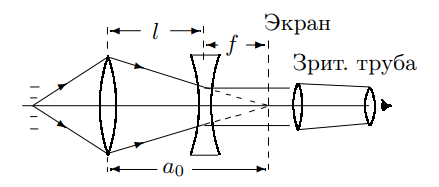
\includegraphics[width=0.6\textwidth]{minus_lens.png}
\end{center}
\caption{Определение фокусного расстояния рассеивающей линзы}
\label{fig:minus_lens}
\end{figure}

\subsection{Телескоп Кеплера}

Из имеющегося набора возьмём линзу 3 в качестве коллиматора, линзы 2 и 1 качестве объектива и окуляра. Настроим коллиматор так же, как в предыдущем пункте. Для последующих расчётов увеличения телескопа измерим размер изображения $h_1$ одного миллиметра шкалы осветителя в делениях шкалы зрительной трубы. $h_1 = k \tan{\alpha_1} \approx k\alpha_1$, где $k$ --- некоторый коэффициент, характеризующий увеличение зрительной трубы, $\alpha_1$ --- угловой размер изображения миллиметрового деления шкалы осветителя, наблюдаемого через коллиматор. Соберём установку, как показано на рис.~\ref{fig:Kepler}.

\begin{figure}[h!]
\begin{center}
    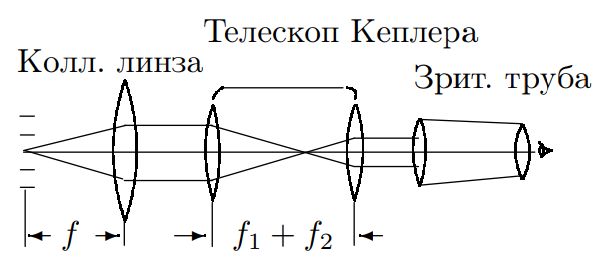
\includegraphics[width=0.7\textwidth]{kepler.png}
\end{center}
\caption{Определение увеличения телескопа Кеплера}
\label{fig:Kepler}
\end{figure}

Рассчитаем увеличение исследуемой модели телескопа через отношения передних фокусных расстояний линз $f_1$, $f_2$ согласно формуле $$N_T = -\frac{f_1}{f_2} = -1,46\pm0,03.$$

Определим увеличение телескопа через отношение углов, под которыми объект виден через телескоп и без него. Для этого найдём размер $h_2$ изображения миллиметрового деления шкалы осветителя в делениях окулярной шкалы зрительной трубы по схеме рис.~\ref{fig:Kepler}. Аналогично, $h_2 = k\tan{\alpha_2} \approx k\alpha_2$, где $\alpha_2$ --- угловой размер изображения миллиметрового деления шкалы при наблюдении через телескоп. Полученные значения: $$h_1 = 10,0\pm0,5~дел, \quad h_2 = 13,0\pm0,5~дел.$$
Определим увеличение по формуле $$N_T = \frac{\alpha_2}{\alpha_1} = -\frac{h_2}{h_1} = -1,3\pm0,1.$$

Определим увеличение телескопа, сравнив диаметр оправы его объектива и диаметр изображения этой оправы в окуляре. Полученные значения $$D_1 = 4,0\pm0,1~см, \quad D_2 = 3,0\pm0,1~см.$$ $$N_T = -\frac{D_1}{D_2} = -1,33\pm0,06.$$

\subsection{Труба Галилея}

Для сборки модели трубы Галилея, в модели телескопа Кеплера вместо собирающей окулярной линзы поставим рассеивающую на расстоянии от объектива, равном разности модулей фокусных расстояний объектива и окуляра. Проведём аналогичные измерения увеличения. В качестве объектива возьмём линзу 4.

Первый способ:
$$N_T = -\frac{f_1}{f_2} = -2,59\pm0,03.$$

Второй способ:
$$h_1 = 10,0\pm0,5~дел, \quad h_2 = 30,0\pm0,5~дел.$$
$$N_T = \frac{\alpha_2}{\alpha_1} = -\frac{h_2}{h_1} = -3,0\pm0,1.$$

\subsection{Модель микроскопа}

Для создания модели микроскопа с увеличением $N_M = 5$ возьмём 2 самые короткофокусные линзы из набора. Рассчитаем необходимые оптический интервал $\vartriangle$ и длину тубуса $l_{12}$ по формулам $$N_M = N_1 N_2, \quad N_1 = -\frac{\vartriangle}{f_1}, \quad N_2 = \frac{L}{f_2}, \quad \vartriangle = l_{12} - f_1 - f_2,$$
где $N_1$, $N_2$ --- увеличения объектива и окуляра, $f_1$, $f_2$ --- положительные передние фокусные расстояния линз, $L = 25~см$ --- расстояние наилучшего зрения. Получаем расчётные значения $\vartriangle = 16,5\pm0,5~см$, $l_{12} = 35,0\pm0,2~см$.

Соберём установку как показано на рис.~\ref{fig:micro}.

\begin{figure}[h!]
\begin{center}
    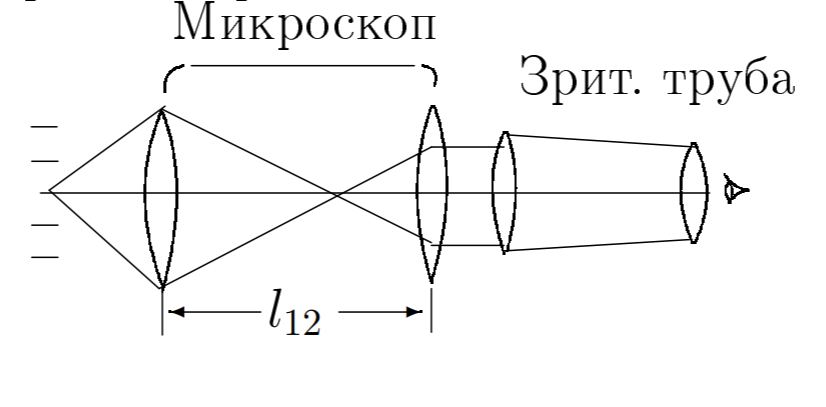
\includegraphics[width=0.7\textwidth]{micro.png}
\end{center}
\caption{Модель микроскопа}
\label{fig:micro}
\end{figure}

Для экспериментального определения увеличения микроскопа измерим величины $h_1$ и $h_2$ так же, как в предыдущих пунктах. Полученные значения: $$h_1 = 18,0\pm0,5~дел, \quad h_2 = 39,0\pm0,5~дел.$$ Рассчитаем увеличение микроскопа по формуле:
$$ N_M = -\frac{h_2}{h_1}\frac{L}{f} = -4,9\pm0,2.$$

\begin{figure}[h!]
\begin{center}
    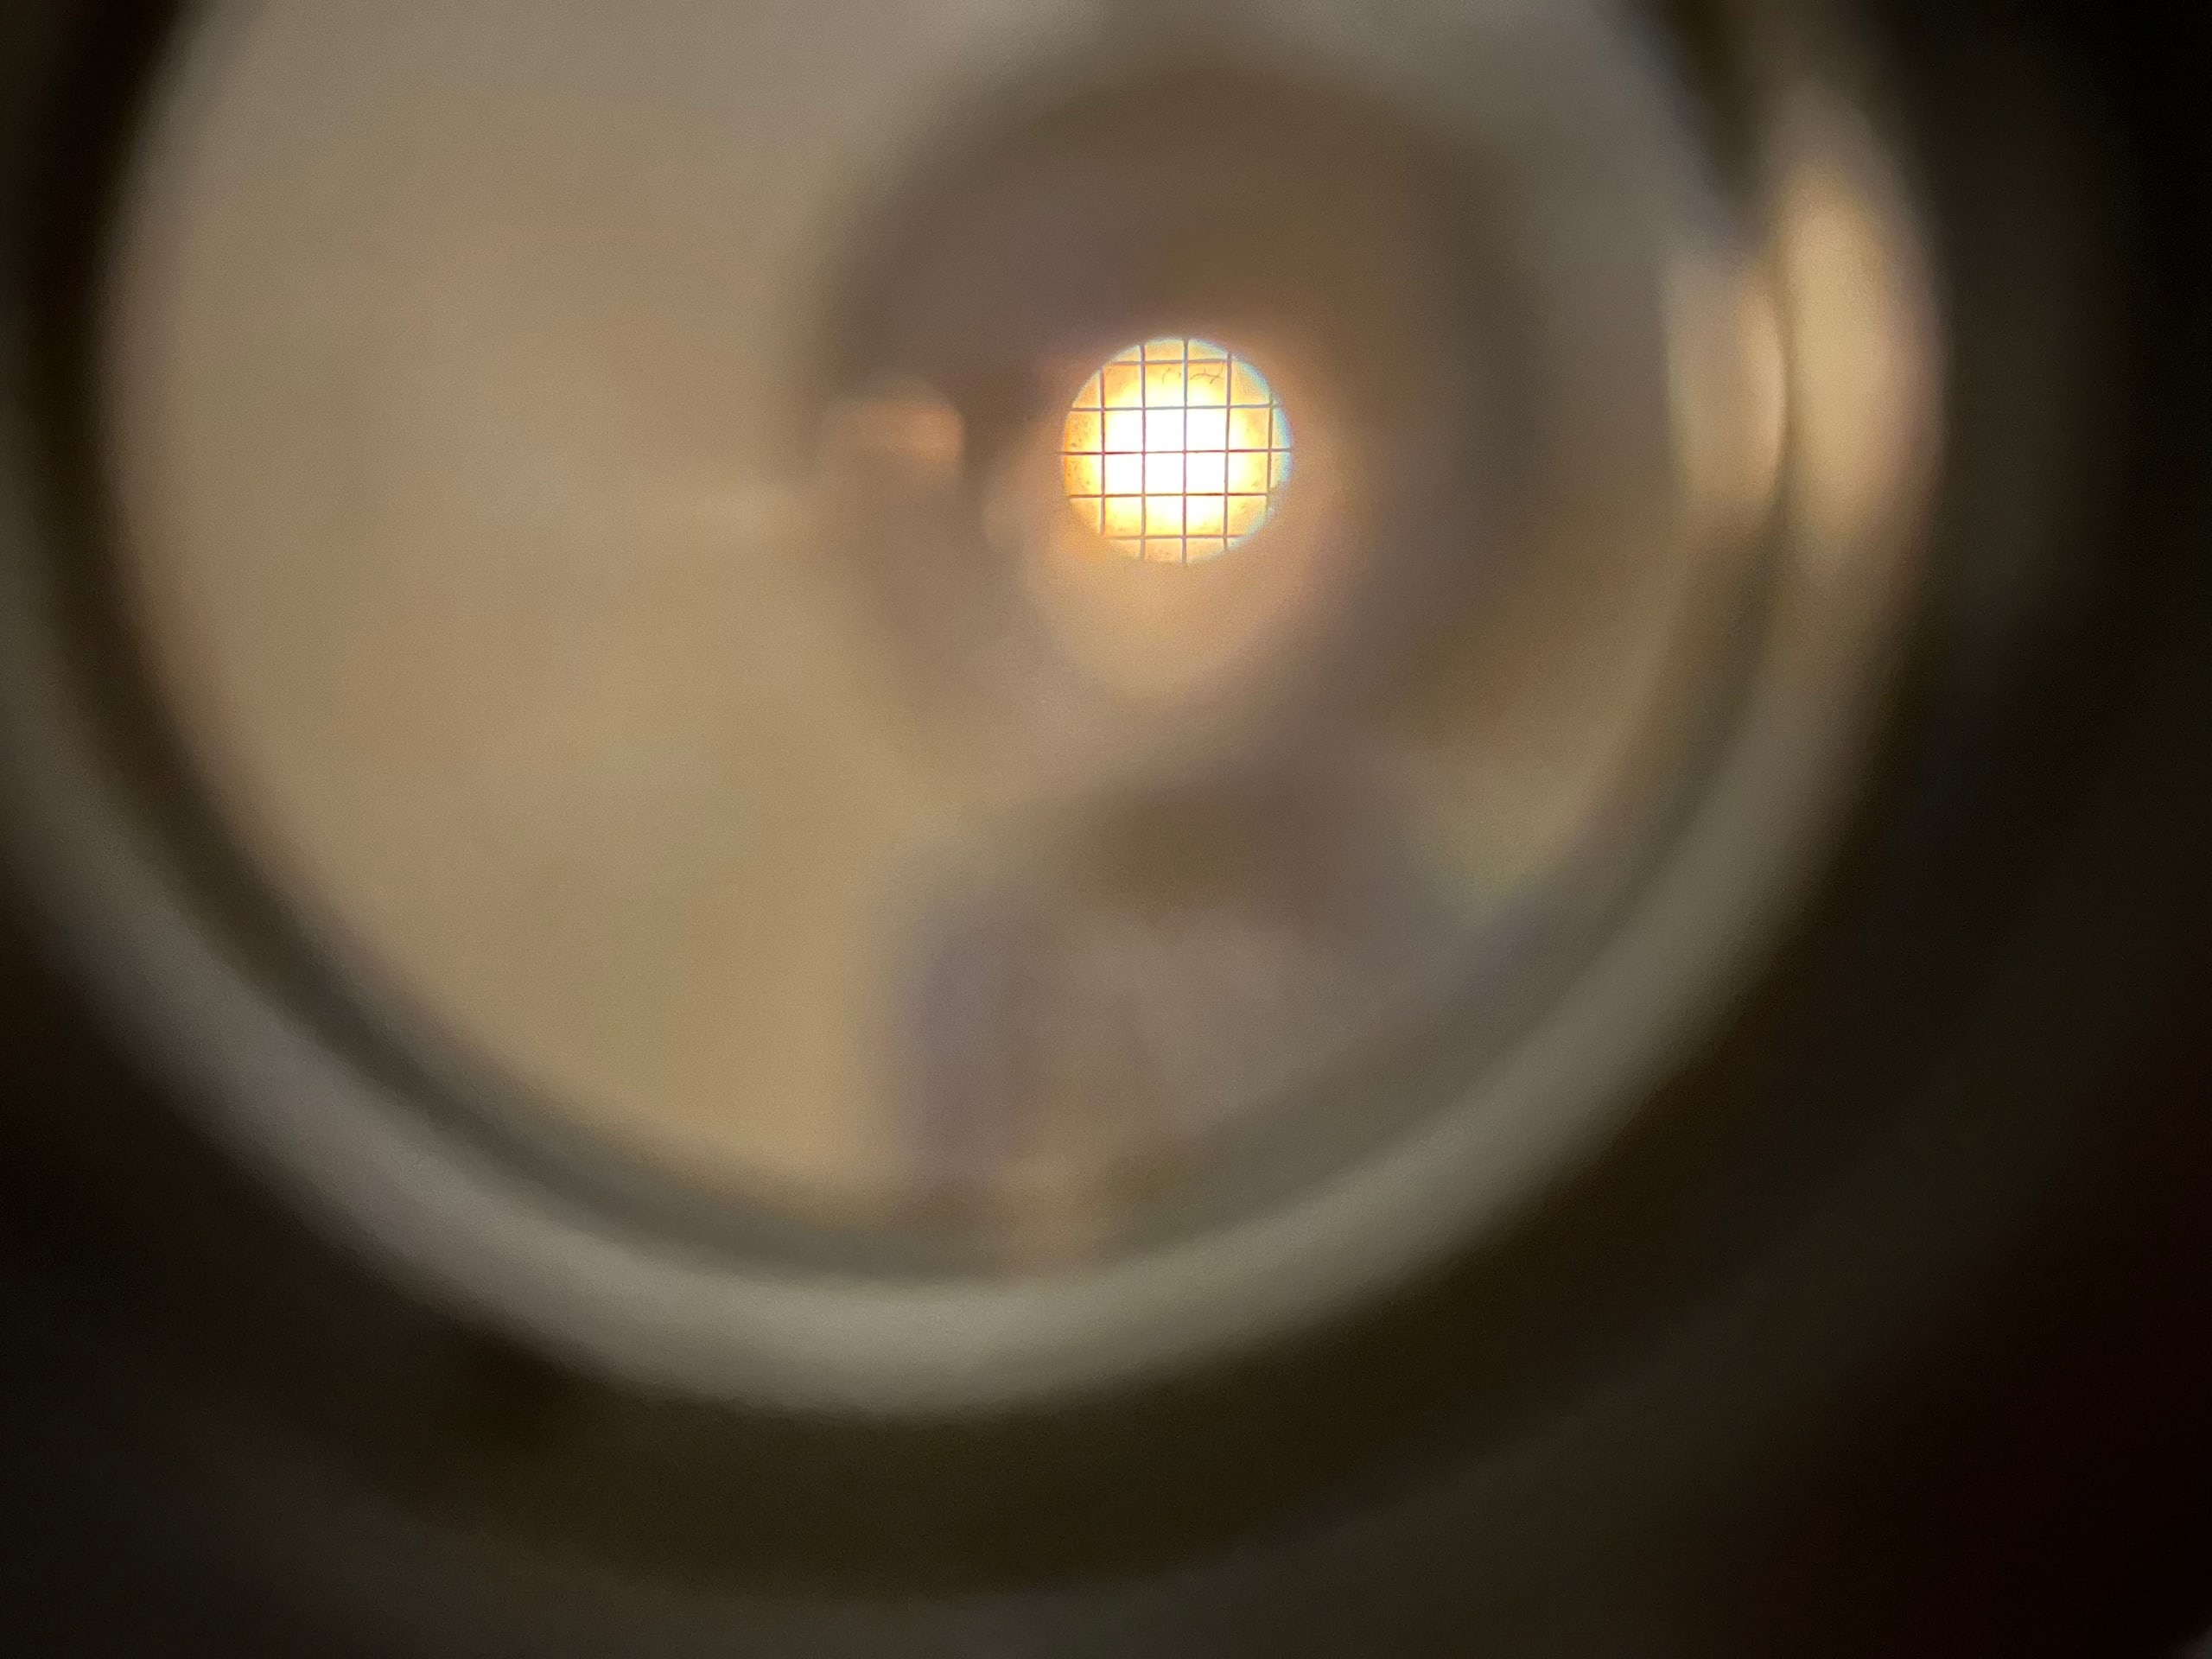
\includegraphics[width=0.5\textwidth]{micro_grid.jpg}
\end{center}
\caption{Шкала осветителя в окуляре микроскопа}
\label{fig:micro_grid}
\end{figure}

\section{Обсуждение результатов и выводы}

В данной работе были исследованы модели зрительных труб и микроскопа. Различными способами были определены их увеличения. Результаты представлены в таб.~\ref{tab:res}.

\begin{table}[h!]
\renewcommand{\arraystretch}{1.5}
\begin{center}
\begin{tabular}{|c|c|c|c|}
\hline
Формула   & Телескоп Кеплера            & Труба Галилея               & Микроскоп                 \\ \hline
$N = -\frac{f_1}{f_2}$     & $-1,46\pm0,03$ & $-2,59\pm0,03$ & $N_M = 5$                  \\ \hline
$N = \frac{\alpha_2}{\alpha_1}$     & $-1,3\pm0,1$  & $-3,0\pm0,1$   & $-4,9\pm0,2$ \\ \hline
$N_T = -\frac{D_1}{D_2}$ & $-1,33\pm0,06$ & ---                           & ---                         \\ \hline
\end{tabular}
\end{center}
\caption{Результаты измерений увеличения оптических приборов}
\label{tab:res}
\end{table}

Результаты всех измерений хорошо согласуются между собой. Наименьшая систематическая погрешность достигается при расчёте увеличения по отношению фокусных расстояний окуляра и объектива. Это связано с небольшой погрешностью определения фокусных расстояний линз. Основной вклад в погрешность других методов вносит погрешность определения размера изображений. Уменьшения погрешности можно достичь более точной юстировкой и центрированием оптической системы.

\end{document}
